%!TEX root = ../paper.tex

\todo[inline]{Mention MSE results}

\begin{figure*}[!ht]
	\centering
	%!TEX root = ../paper.tex

% Ferdosi 1 - MBE
\begin{subfigure}{0.23\textwidth}
	\centering
	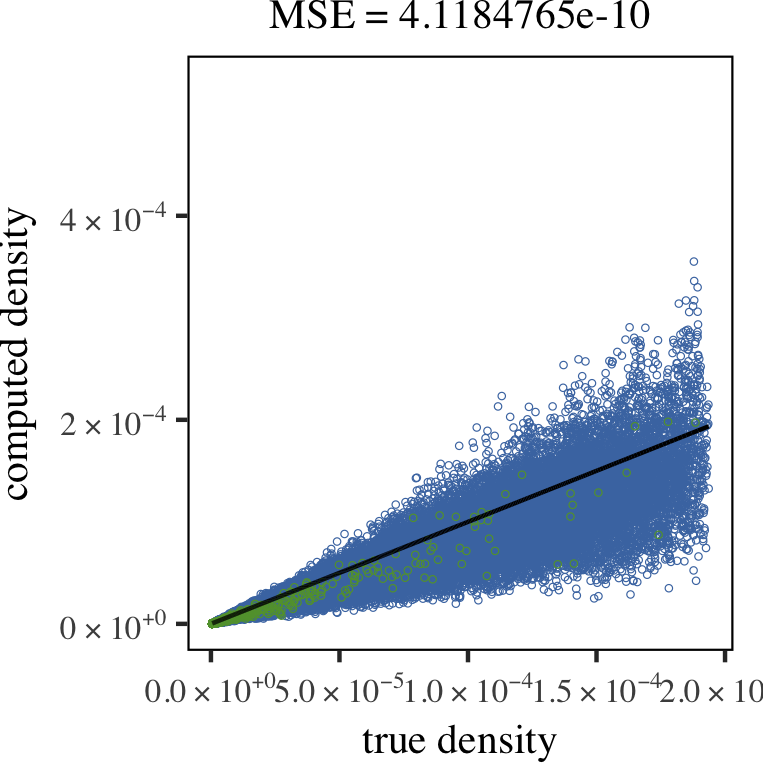
\includegraphics[keepaspectratio=true, width=\textwidth, height=0.23\textheight]{result/img/all/results_ferdosi_1_60000_mbe_silverman}
	\caption{Set \ferdosiOne, \mbe}
	\label{fig:results:singlesphere:mbe:ferdosi1}
\end{subfigure}
% Baakman 1	- MBE
\begin{subfigure}{0.23\textwidth}
	\centering
	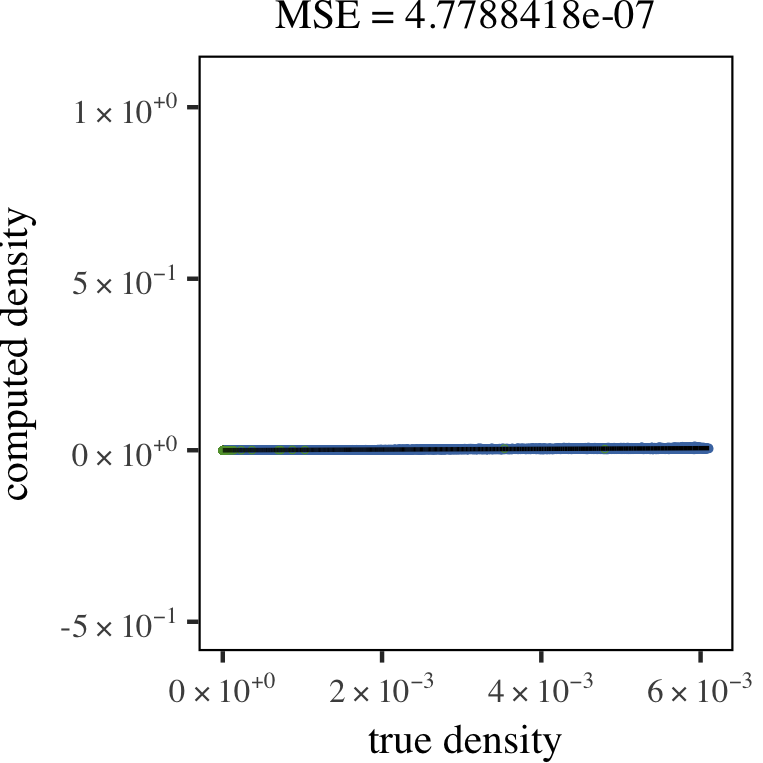
\includegraphics[keepaspectratio=true, width=\textwidth, height=0.23\textheight]{result/img/all/results_baakman_1_60000_mbe_silverman}
	\caption{Set \baakmanOne, \mbe}
	\label{fig:results:singlesphere:mbe:baakman1}
\end{subfigure}
% Baakman 4 - MBE
\begin{subfigure}{0.23\textwidth}
	\centering
	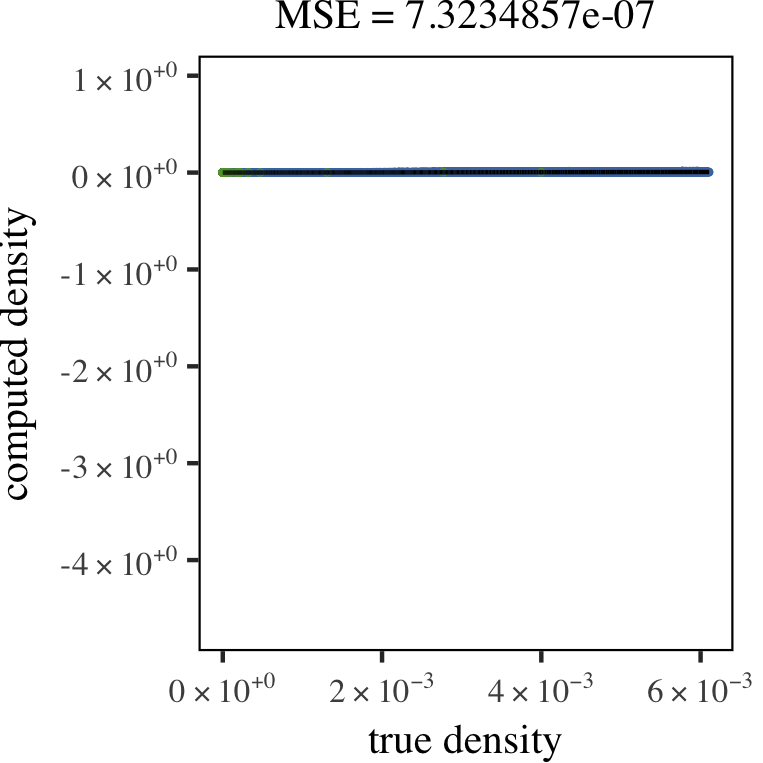
\includegraphics[keepaspectratio=true, width=\textwidth, height=0.23\textheight]{result/img/all/results_baakman_4_60000_mbe_silverman}
	\caption{Set \baakmanFour, \mbe}
	\label{fig:results:singlesphere:mbe:baakman4}
\end{subfigure}	
% Baakman 5 - MBE
\begin{subfigure}{0.23\textwidth}
	\centering
	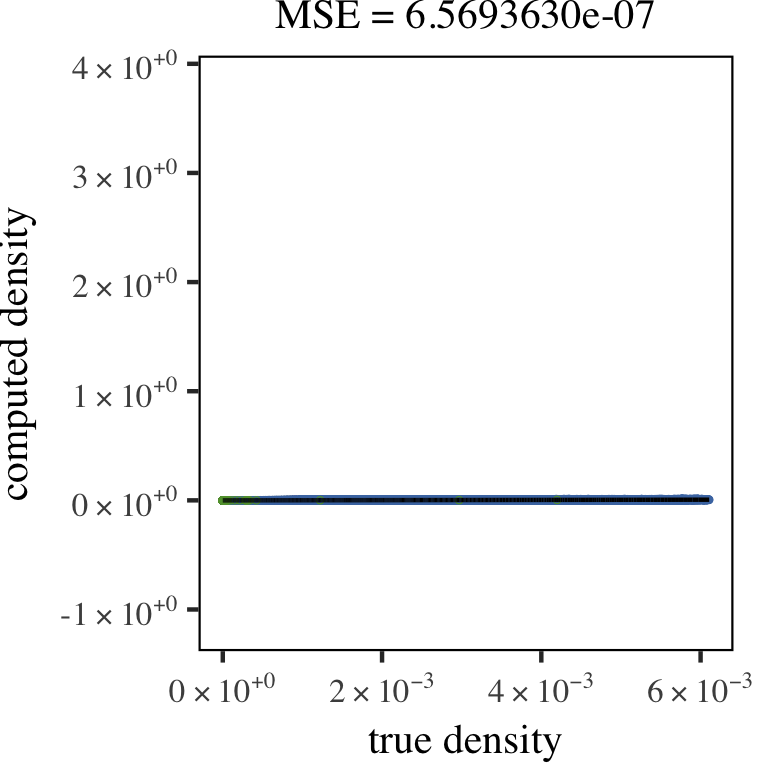
\includegraphics[keepaspectratio=true, width=\textwidth, height=0.23\textheight]{result/img/all/results_baakman_5_60000_mbe_silverman}
	\caption{Set \baakmanFive, \mbe}
	\label{fig:results:singlesphere:mbe:baakman5}
\end{subfigure}
% Ferdosi 1 - SAMBE
\begin{subfigure}{0.23\textwidth}
	\centering
	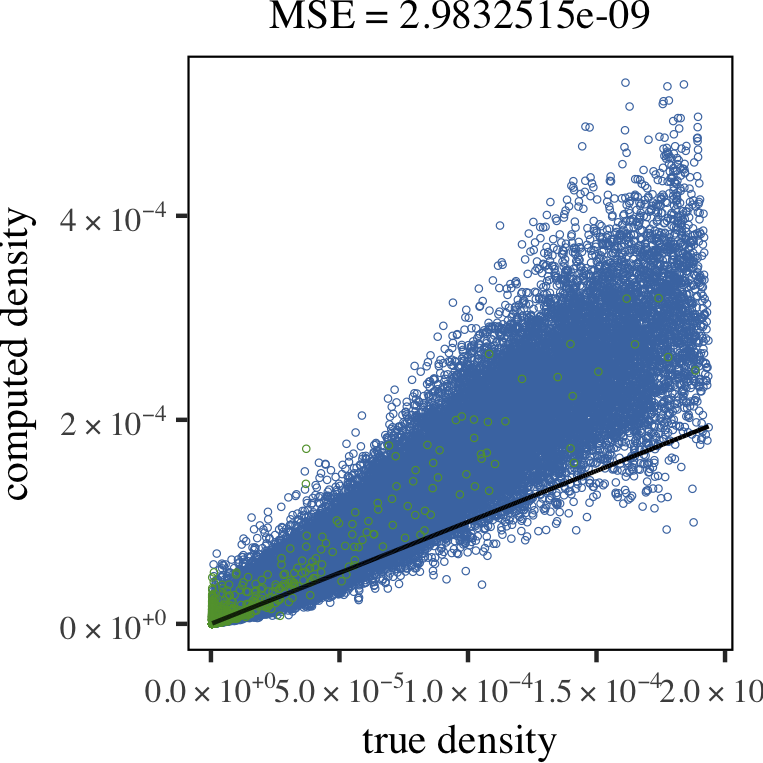
\includegraphics[keepaspectratio=true, width=\textwidth, height=0.23\textheight]{result/img/all/results_ferdosi_1_60000_sambe_silverman}
	\caption{Set \ferdosiOne, \sambe}
	\label{fig:results:singlesphere:sambe:ferdosi1}
\end{subfigure}
% Baakman 1	- SAMBE
\begin{subfigure}{0.23\textwidth}
	\centering
	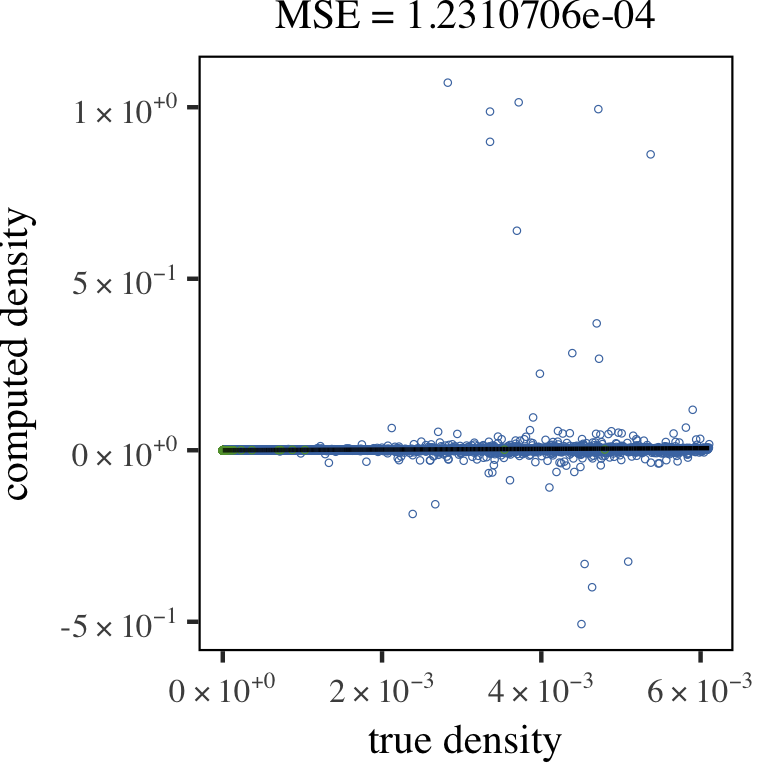
\includegraphics[keepaspectratio=true, width=\textwidth, height=0.23\textheight]{result/img/all/results_baakman_1_60000_sambe_silverman}
	\caption{Set \baakmanOne, \sambe}
	\label{fig:results:singlesphere:sambe:baakman1}
\end{subfigure}
% Baakman 4 - SAMBE
\begin{subfigure}{0.23\textwidth}
	\centering
	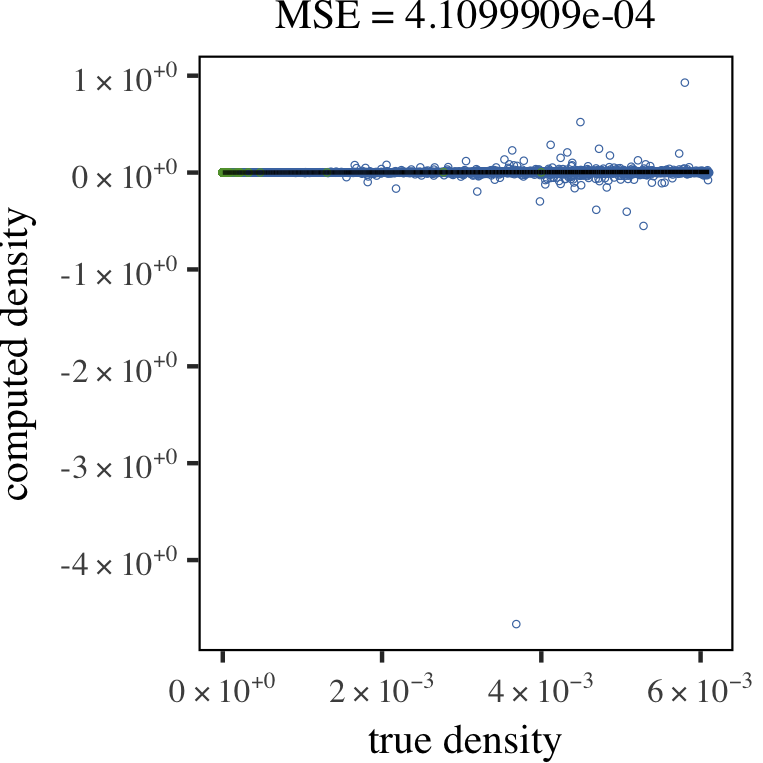
\includegraphics[keepaspectratio=true, width=\textwidth, height=0.23\textheight]{result/img/all/results_baakman_4_60000_sambe_silverman}
	\caption{Set \baakmanFour, \sambe}
	\label{fig:results:singlesphere:sambe:baakman4}
\end{subfigure}		
% Baakman 5 - SAMBE
\begin{subfigure}{0.23\textwidth}
	\centering
	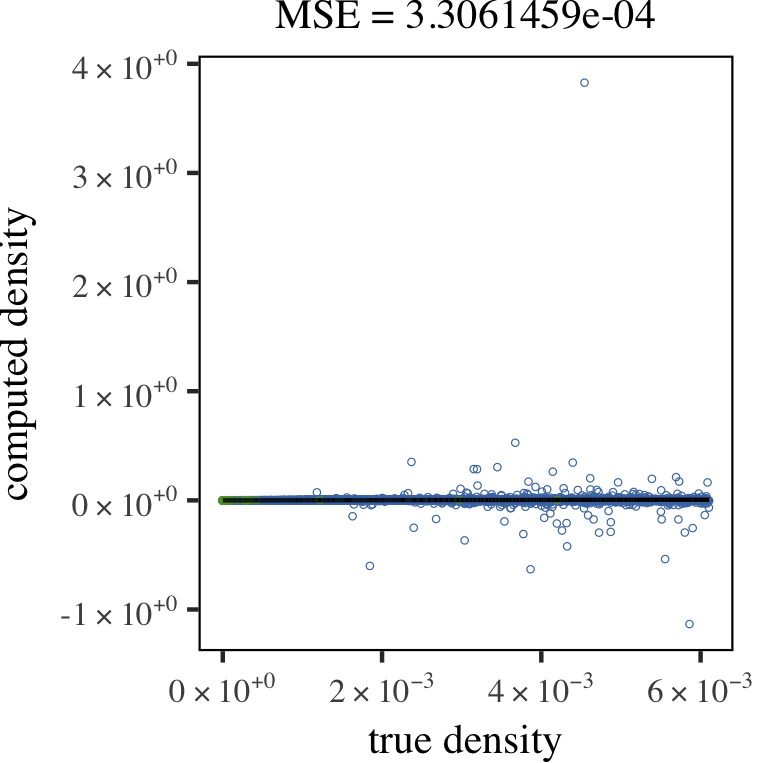
\includegraphics[keepaspectratio=true, width=\textwidth, height=0.23\textheight]{result/img/all/results_baakman_5_60000_sambe_silverman}
	\caption{Set \baakmanFive, \sambe}
	\label{fig:results:singlesphere:sambe:baakman5}
\end{subfigure}	
	\caption{Comparative plots for dataset \ferdosiOneNum, \baakmanOneNum, \baakmanFourNum, and \baakmanFiveNum.
	}
	\label{fig:4:results:singleSphere}
\end{figure*}

%PLOT results
	\Cref{fig:4:results:singleSphere} presents the results of using the Modified Breiman Estimator and its shape adaptive variant to estimate the densities of the datasets in \cref{tab:3:simulated:datasets} that contain a single Gaussian distribution. 

	% Ferdosi 1
		\Cref{fig:4:results:mbe:ferdosi1} confirms our findings from \cref{s:results:mse}, namely that the Modified Breiman Estimator gives a good approximation of the densities of dataset \ferdosiOne. The densities estimated with the \mbe both over, and undershoot the true density. \Cref{fig:4:results:mbe:ferdosi1}, on the other hand, shows that shape adaptive \mbe nearly always overshoots the true density. 

	% Baakman 1
		% Normal Plot
		Comparing the performance of the two estimators on dataset \baakmanOne with \cref{fig:4:results:mbe:baakman1,fig:4:results:sambe:baakman1} we find that the Modified Breiman Estimator outperforms the shape-adaptive variant. The second estimator has some extreme outliers, the most extreme of which are \num{1.071674654143224}, and \num{-0.506829052779317}. 
		% No Outlier Plot
		% Plotting only the results where the densities as estimated by \sambe are in the range $\left(\num{0.0}, \num[round-precision=1]{0.07} \right)$ results in \Cref{fig:results:baakman1:noOutliers}. Observing \cref{fig:results:baakman1::noOUtliers:sambe} we find that the shape-adaptive estimator results in a great spread of densities than the non-shape adaptive variant. However the densities that fall within the range $\left(\num[round-precision=1]{0.0}, \num[round-precision=1]{0.07} \right)$ are reasonable approximates of the true density. The smaller range of \cref{fig:4:results:mbe:baakman1} shows that the \mbe does not result in a perfect estimate, as \cref{fig:results:baakman1:noOutliers:mbe} suggest, but that the approximation is good, as indicated by the MSE.
		% \begin{figure}[!ht]
		% 	\centering
		% 	\begin{subfigure}{0.6\columnwidth}
		% 		\centering
		% 		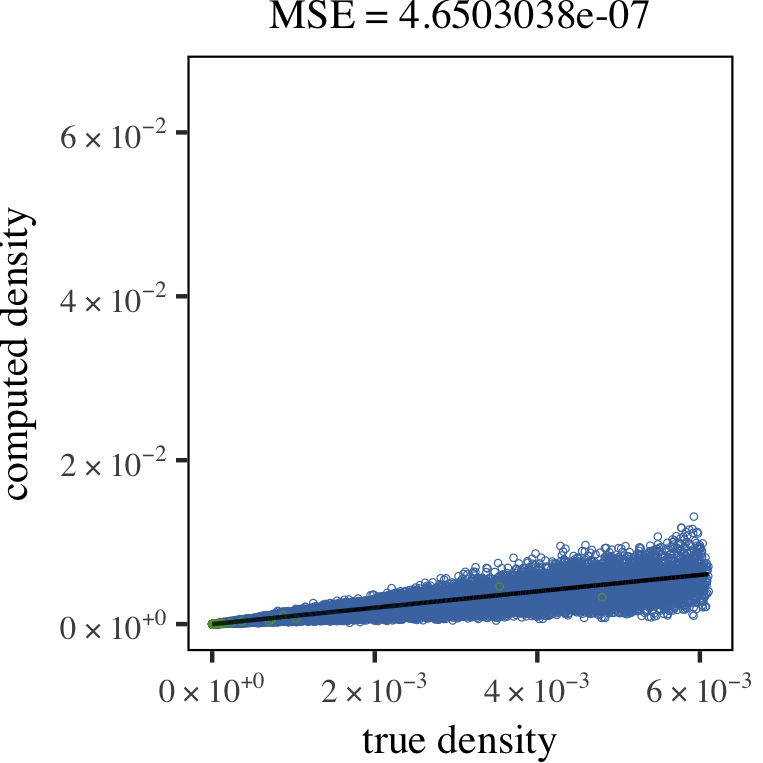
\includegraphics[width=\textwidth]{result/img/noOutliers/results_baakman_1_60000_mbe_silverman_no_outliers.png}
		% 		\caption{\mbe}
		% 		\label{fig:results:baakman1:noOutliers:mbe}
		% 	\end{subfigure}
		% 	\begin{subfigure}{0.6\columnwidth}
		% 		\centering
		% 		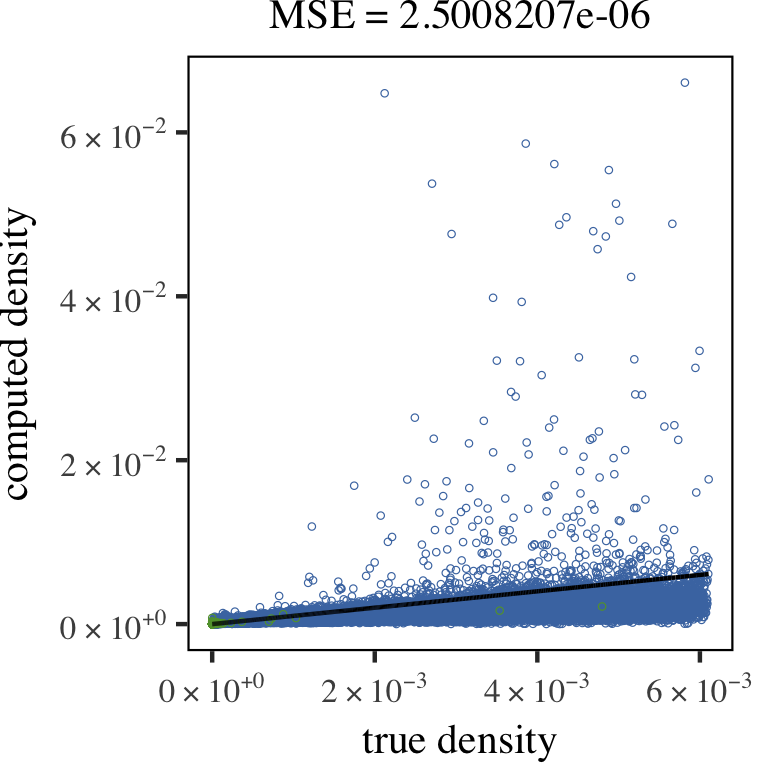
\includegraphics[width=\textwidth]{result/img/noOutliers/results_baakman_1_60000_sambe_silverman_no_outliers.png}
		% 		\caption{\sambe}
		% 		\label{fig:results:baakman1::noOUtliers:sambe}
		% 	\end{subfigure}	
		% 	\caption{Comparative plots between the true densities of dataset \baakmanOneNum\xspace as estimated by \subref{fig:results:baakman1:noOutliers:mbe} \mbe and \subref{fig:results:baakman1::noOUtliers:sambe} \sambe, with only the points whose density is estimated by \sambe to lie in $\left(\num{0.0}, \num[round-precision=1]{0.07} \right)$.}
		% 	\label{fig:results:baakman1:noOutliers}
		% \end{figure}

	% Baakman 4
		% Normal Plot
		The results of data set \baakmanFour, shown in \cref{fig:4:results:mbe:baakman1,fig:4:results:sambe:baakman1} respectively, are comparable to those of \baakmanOne: the original estimator approximates the density pretty well, the shape-adaptive variant has some extreme outliers, the densities estimated by \sambe fall in the range, $\left[\num{-4.660977565610216}, \num{0.928287124473193}\right]$, whereas the true densities all lie within $\left[\num[scientific-notation=true]{0.000000500000000}, \num[scientific-notation=true]{0.006107784664258}\right]$.
		% No Outlier Plot
		% \Cref{fig:results:baakman4:noOutliers} presents the comparative plots for \mbe and \sambe for dataset \baakmanFour without patterns with estimated densities outside the range $\left(\num{0.0}, \num[round-precision=2]{0.15} \right)$. The results illustrated in this figure are comparable to those of \cref{fig:results:baakman1:noOutliers}: for a number of points the densities are overestimated, but otherwise the estimated densities seem reasonable.	

		% \begin{figure}
		% 	\centering
		% 	\begin{subfigure}{0.6\columnwidth}
		% 		\centering
		% 		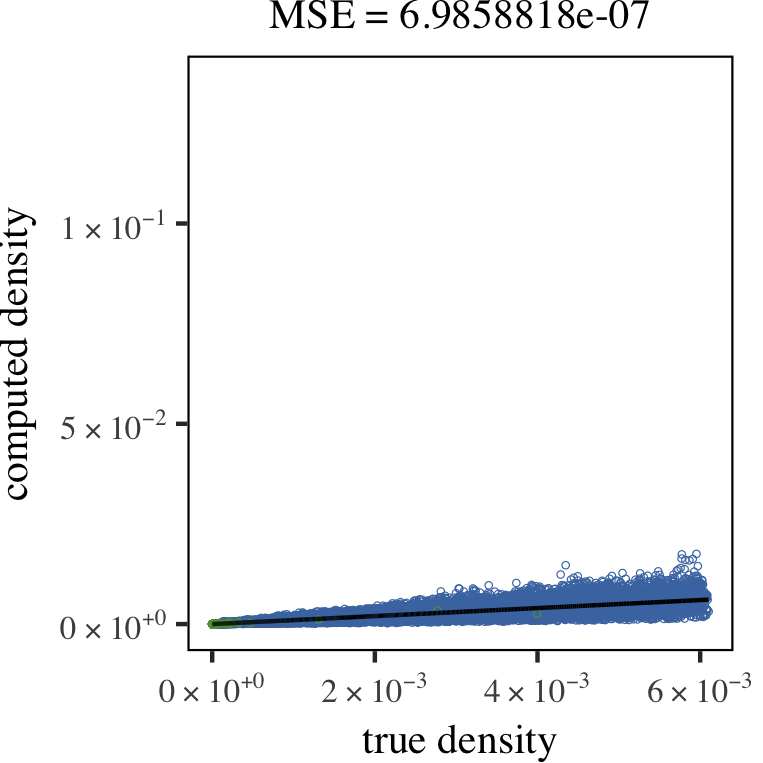
\includegraphics[width=\textwidth]{result/img/noOutliers/results_baakman_4_60000_mbe_silverman_no_outliers.png}
		% 		\caption{\mbe}
		% 		\label{fig:results:baakman4:noOutliers:mbe}
		% 	\end{subfigure}
		% 	\begin{subfigure}{0.6\columnwidth}
		% 		\centering
		% 		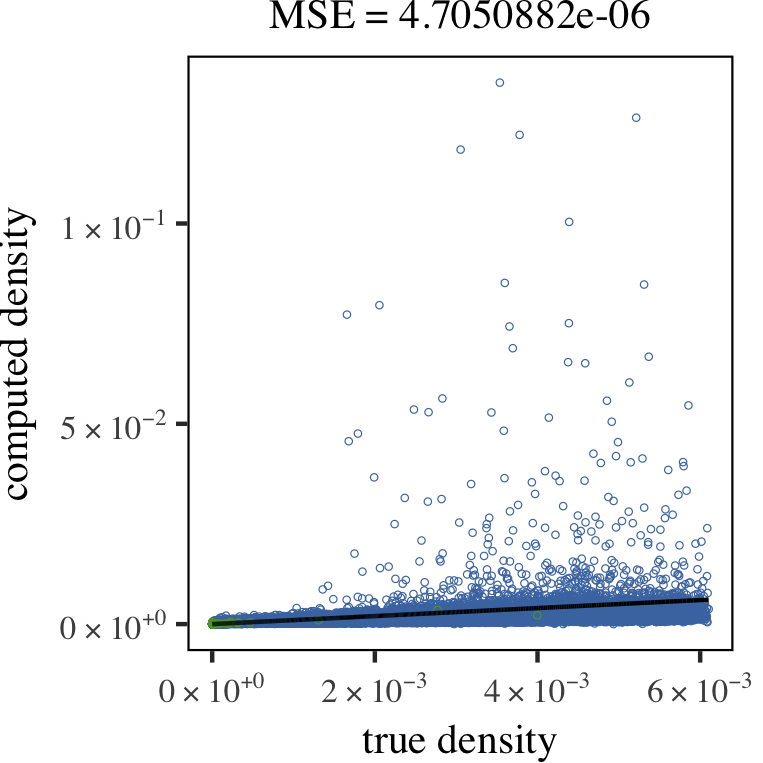
\includegraphics[width=\textwidth]{result/img/noOutliers/results_baakman_4_60000_sambe_silverman_no_outliers.png}
		% 		\caption{\sambe}
		% 		\label{fig:results:baakman4:noOUtliers:sambe}
		% 	\end{subfigure}	
		% 	\caption{Comparative plots between the true densities of dataset \baakmanFourNum\xspace as estimated by \subref{fig:results:baakman4:noOutliers:mbe} \mbe and \subref{fig:results:baakman4:noOUtliers:sambe} \sambe, with only the points whose density is estimated by \sambe to lie in $\left(\num{0.0}, \num{0.15} \right)$.}
		% 	\label{fig:results:baakman4:noOutliers}
		% \end{figure}

	% Baakman 5
		% Normal Plot
		\Cref{fig:4:results:mbe:baakman5,fig:4:results:sambe:baakman5} compare the performance of respectively \mbe with \sambe on data set \baakmanFive. We once again observe that the non-shape adaptive estimator approximates the known densities pretty well. Whereas the shape-adaptive estimator returns extreme results with densities that are estimated to be as high as \num{3.827317431934174} and as low as \num{-1.133853887375073}.
		%OutlierPlot
		% Removing all patterns which have a density that is estimated by \sambe to lie outside the range $\left(\num{0.0}, \num[round-precision=2]{0.3} \right)$ results in \cref{fig:results:baakman5:noOutliers}. Comparing \cref{fig:results:baakman5:noOutliers:mbe} with \cref{fig:results:baakman5:noOUtliers:sambe} leads to the same conclusion as drawn about dataset \baakmanOne and \baakmanFour.

		% \begin{figure}
		% 	\centering
		% 	\begin{subfigure}{0.6\columnwidth}
		% 		\centering
		% 		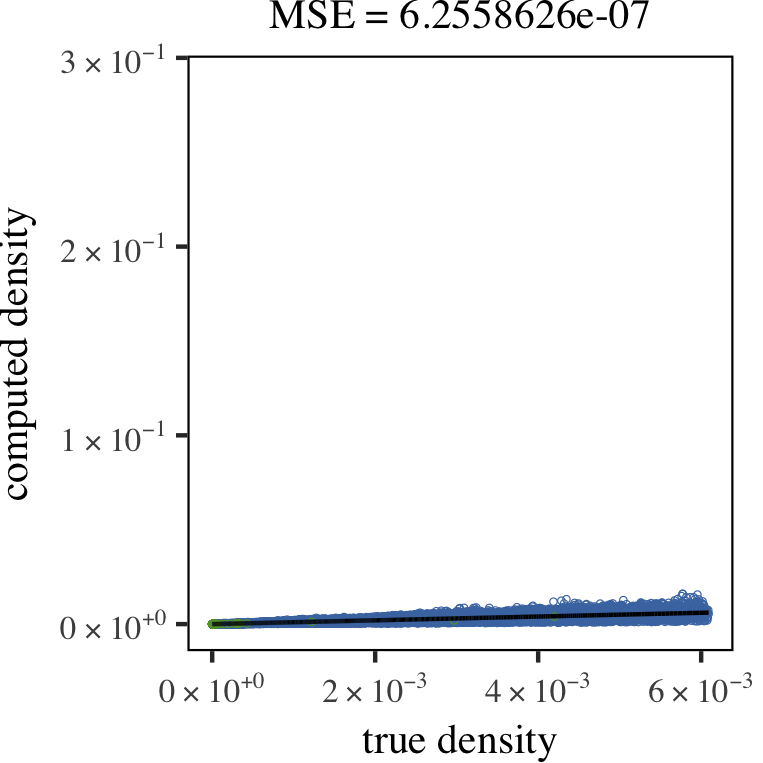
\includegraphics[width=\textwidth]{result/img/noOutliers/results_baakman_5_60000_mbe_silverman_no_outliers.png}
		% 		\caption{\mbe}
		% 		\label{fig:results:baakman5:noOutliers:mbe}
		% 	\end{subfigure}
		% 	\begin{subfigure}{0.6\columnwidth}
		% 		\centering
		% 		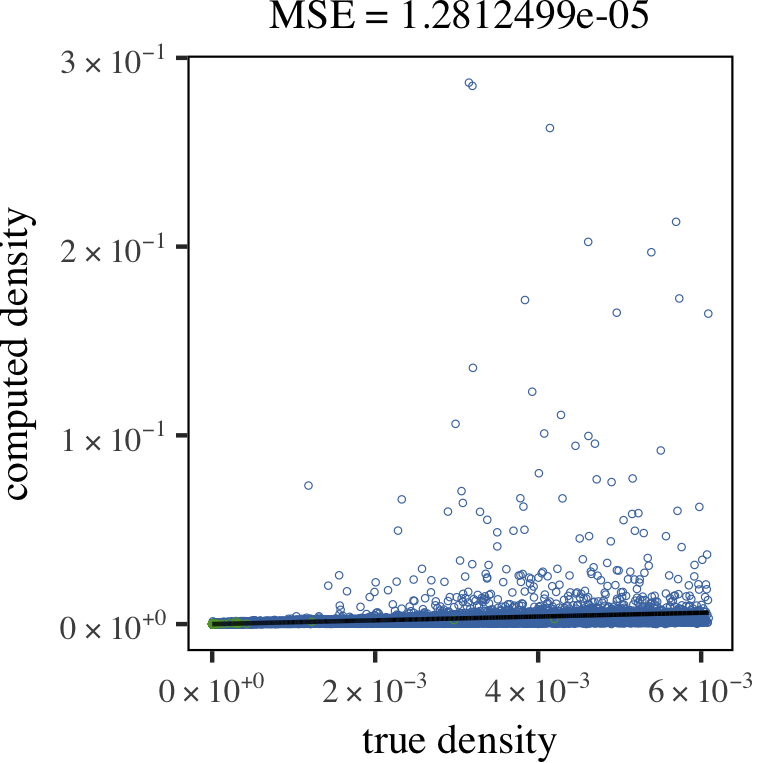
\includegraphics[width=\textwidth]{result/img/noOutliers/results_baakman_5_60000_sambe_silverman_no_outliers.png}
		% 		\caption{\sambe}
		% 		\label{fig:results:baakman5:noOUtliers:sambe}
		% 	\end{subfigure}	
		% 	\caption{Comparative plots between the true densities of dataset \baakmanFiveNum as estimated by \subref{fig:results:baakman5:noOutliers:mbe} \mbe and \subref{fig:results:baakman5:noOUtliers:sambe} \sambe, with only the points whose density is estimated by \sambe to lie in $\left(\num{0.0}, \num{0.15} \right)$.}
		% 	\label{fig:results:baakman5:noOutliers}
		% \end{figure}

	% Algehele observatie voor single sphere datsets
		% MBE beter dan SAMBE
		In general we have found that the Modified Breiman estimator works pretty well for data sets that contain a single Gaussian, especially if the Gaussian is spherical. Since the mean square error for dataset \baakmanFive is lower than the MSE of dataset \baakmanFour the ellipticalness of the distribution does not seem to influence the performance of this estimator. 
		% Hoe elongated heeft geen invloed
		The shape adaptive \mbe results in some extremely high and low estimated densities if used to estimate the densities of non-spherical Gaussian. \sambe overestimated some of the densities of the spherical Gaussian compared to the Modified Breiman Estimator. The range of the values estimated by the shape-adaptive estimator does not seem to be influenced by how electricalness of the Gaussian distribution. 
		% Removing OUtliers
		% \todo[inline]{Schrijf iets over resulaten als de outliers eruit zijn.}